\begin{hint}{Achtung!}{unvollstaendig-som}
	Dieser Abschnitt der Zusammenfassung ist sehr wahrscheinlich unvollständig und sollte überarbeitet werden!
	Aus Zeitgründen wurden hier nicht alle Themen der Vorlesung erarbeitet.
	\begin{flushright}\textit{Beni}\end{flushright}
\end{hint}
\noindent
Die selbstorganiserenden Karten (engl. self-organizing maps (SOM), auch Kohonen Maps oder Kohonen Feature Maps) sind eng verwand mit der lernenden Vektorquantisierung (LVQ). Man kann sie als Weiterentwicklung von LVQ unter Betrachtung einer \emph{lokalen Nachbarschaftsbeziehung} der Neuronen betrachten.


% ------------------------------------------------------------------------
% ------------------------------------------------------------------------
\section*{Prinzip}
Bei den selbstorganisierenden Karten handelt es sich wieder um einschichtige neuronale Netze mit einer Schicht aktiver Neuronen. Die selbstorganisierenden Karten werden im Gegensatz zu LVQ aber mit \emph{unüberwachten} Lernverfahren trainiert.

Die Ausgabe der SOMs ist deren Zustand: Es ist nicht interessant, was die Neuronen berechnen und ausgeben, sondern nur welches Neuron gerade aktiv ist. Damit sind SOMs wesentlich biologieverwandter als beispielsweise feedforward-Netze.



% ------------------------------------------------------------------------
% ------------------------------------------------------------------------
\section*{Aufbau}
SOMs haben - wie das Gehirn - typischerweise die Aufgabe, einen hochdimensionalen Input ($N$ Dimensionen) auf Bereiche in einem niedrigdimensionalen Gitter ($G$ Dimensionen) abzubilden, also sozusagen eine \emph{Karte} von dem hochdimensionalen Raum zu zeichnen. Um diese Karte zu erschaffen, erhält die SOM einfach beliebig viele Punkte aus dem Inputraum.
Die SOM wird während der Eingabe der Punkte versuchen, die Orte, auf denen die Punkte auftreten, so gut wie möglich mit ihren Neuronen abzudecken. Dies bedeutet insbesondere, dass jedes Neuron einem bestimmten Ort im Inputraum zuzuordnen ist.

Es gibt damit zwei Räume, in denen SOMs arbeiten:
\begin{itemize}
	\item \emph{N-dimensionaler Eingaberaum}
	\item \emph{G-dimensionales Gitter} - Stellt die Nachbarschaftsbeziehungen der Neuronen und damit die Netztopologie dar. 
\end{itemize}

Wichtig: Auch dann, wenn $N = G$ gilt, sind die beiden Räume nicht gleich und müssen unterschieden werden. Sie haben in diesem Spezialfall nur die gleiche Dimension.

\subsection*{Gitterstruktur}
Folgende Gitterstrukturen sind üblich:
\begin{itemize}
	\item \emph{eindimensionale} Gitter - Anordnung wie bei einer Perlenkette (siehe Abbildung ? oben). Jedes Neuron besitzt genau zwei Nachbarn (außer die beiden Endneuronen).
	\item \emph{zweidimensionale} Gitter - Rechtwinklige (siehe Abbildung ? unten) oder wabenförmige Anordnungen. Auch ungleichmäßige Topologien sind möglich, jedoch nicht sehr häufig.
	\item \emph{mehrdimensionale} Gitter - Topologien mit mehr Dimensionen und wesentlich mehr Nachbarschaftsbeziehungen wären auch denkbar, werden aber aufgrund der mangelnden Visualisierungsfähigkeit nicht oft eingesetzt.
\end{itemize}

\begin{figure}[ht!] \centering 
	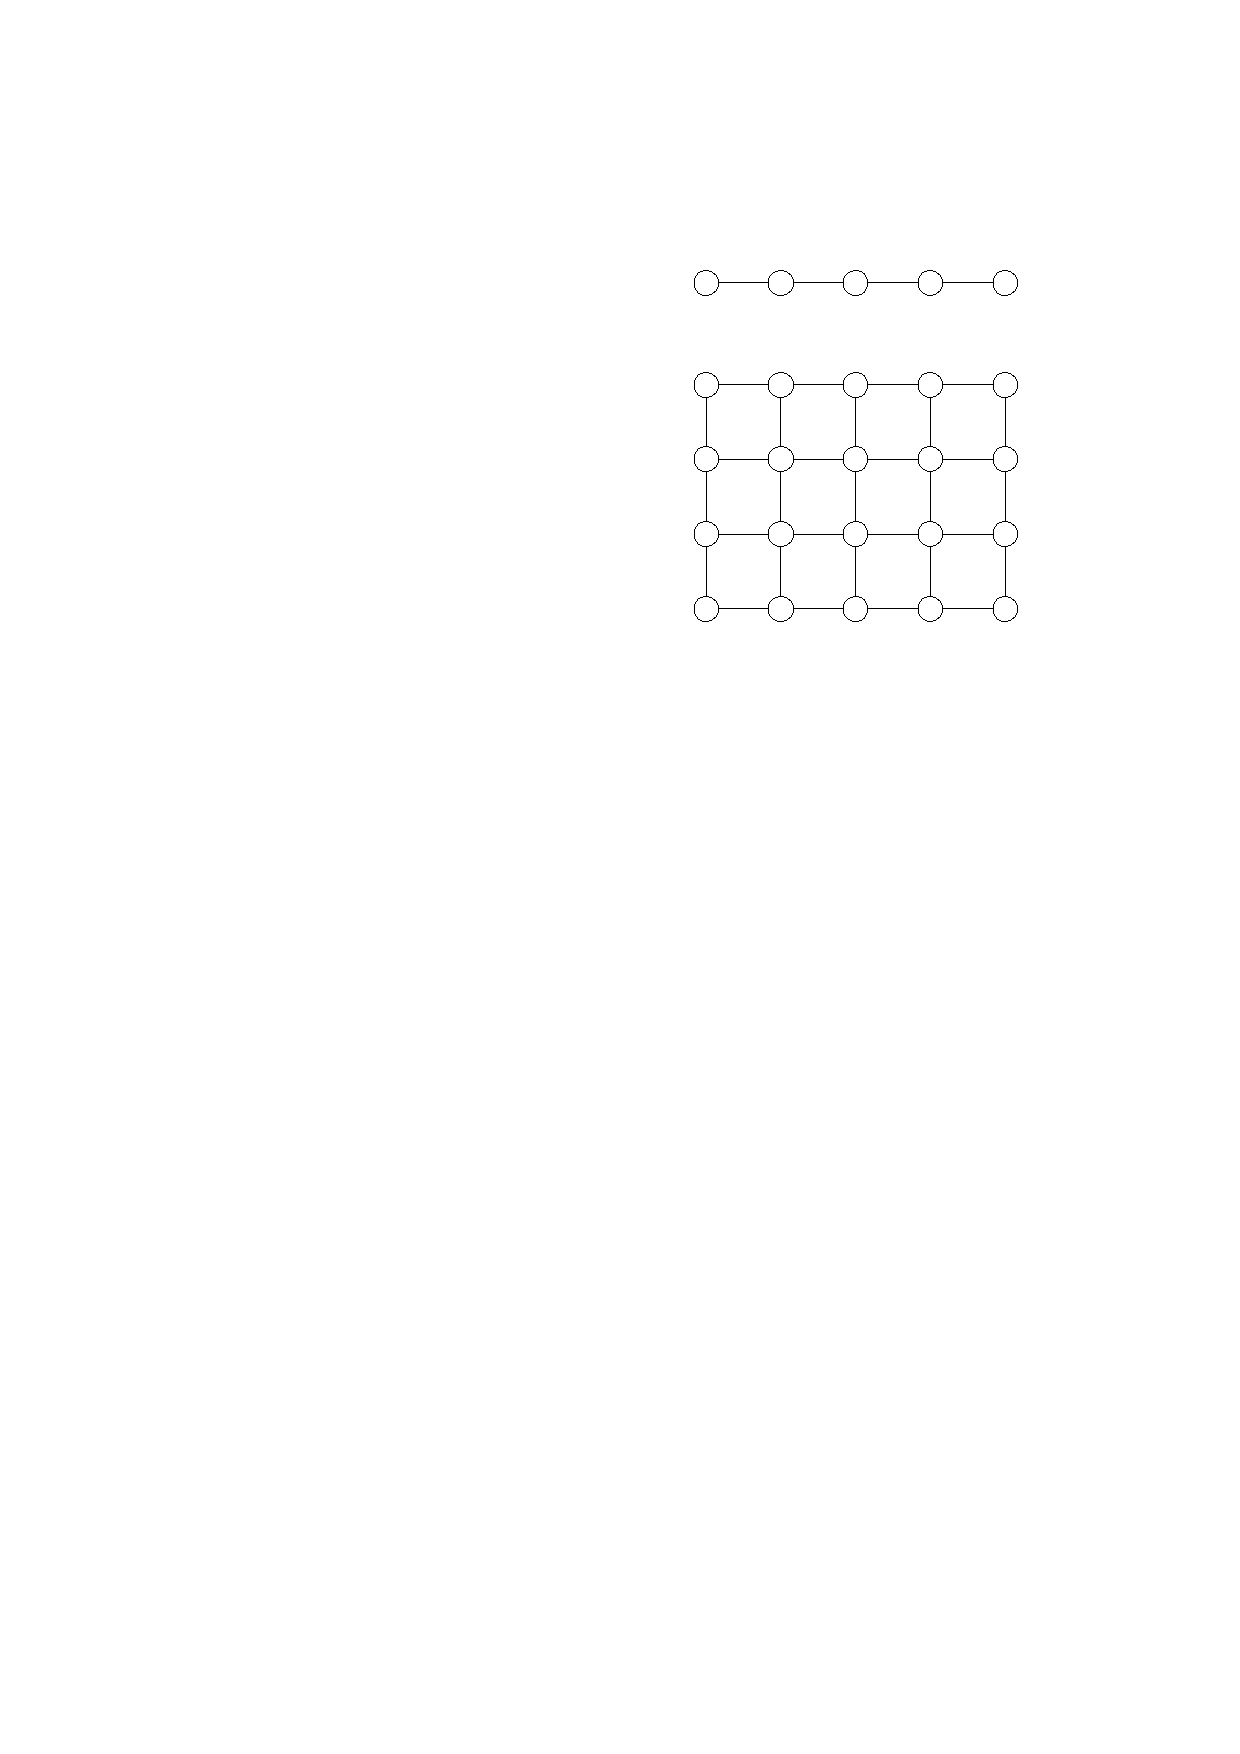
\includegraphics[width=0.5\linewidth]{figures/ch08_som-gitter.pdf}
	\caption{Beispieltopologien einer Self Organizing Map - Oben eine eindimensionale Topologie, unten eine zweidimensionale.}
	\label{fig:ch08_som-gitter}
\end{figure}


\subsection*{SOM-Neuron}
Ein SOM-Neuron $k$ besitzt eine feste Position $c_k$ (\emph{Zentrum} genannt) im Eingaberaum.


\subsection*{SOM}
Eine Self Organizing Map ist eine Menge $K$ von SOM-Neuronen. Bei Eingabe eines Eingabevektors wird genau dasjenige Neuron $k \in K$ aktiv, welches dem Eingabemuster im Eingaberaum am nächsten liegt.


\subsection*{Topologie}
Die Neuronen sind untereinander durch Nachbarschaftsbeziehungen verbunden. Diese Beziehungen nennt man \emph{Topologie}. Sie nimmt starken Einfluss auf das Training einer SOM und wird durch die Topologiefunktion $h(i,k,t)$ definiert.
Dabei ist $i$ das Gewinnerneuron, $k$ das gerade zu adaptierende Neuron und $t$ der Zeitschritt.


% ------------------------------------------------------------------------
% ------------------------------------------------------------------------
\section*{Funktionsweise}
Die Funktionsweise eine SOM teilt sich in die folgenden Schritte auf:

\begin{itemize}
	\item \emph{Eingabe} - Beliebiger Wert $p$ aus dem Eingaberaum $\mathbb{R}^N$.
	\item \emph{Abstandsberechnung} - Es wird der Abstand von jedem SOM-Neuron $k$ zur Eingabe $p$ berechnet: $||p - c_k||$
	\item \emph{Aktivierung} - \emph{Ein} Neuron wird aktiv, nämlich genau das Neuron $i$ mit dem kürzesten zuvor berechneten Abstand zur Eingabe $p$. Alle anderen Neuronen sind inaktiv (\emph{Winner-Takes-All-Schema}).
	\item \emph{Ausgabe} - Die Ausgabe der SOM ist \emph{welches} Neuron aktiv ist. 
\end{itemize}


% ------------------------------------------------------------------------
% ------------------------------------------------------------------------
\section*{Training}
Die Frage des Trainings ist, welches SOM-Neuron $k$ bei welcher Eingabe $p$ aktiv wird.

Das Training einer SOM unterteilt sich in fünf (zum Teil der Funktionsweise recht ähnliche) Schritte:

\begin{enumerate}
	\item \emph{Initialisierung} - Start des Netzes mit zufälligen Neuronenzentren $c_k \in \mathbb{R}^N$ aus dem Eingaberaum.
	\item \emph{Anlegen eines Eingabemusters} - Es wird ein Punkt $p$ aus dem Eingaberaum $\mathbb{R}^N$ (auch \emph{Stimulus} genannt) gewählt und in das Netz eingegeben.
	\item \emph{Abstandsmessung} - Für jedes SOM-Neuron $k$ im Netz wird nun der Abstand $||p - c_k||$ bestimmt.
	\item \emph{Winner takes all} - Es wird das \emph{Gewinnerneuron} $i$ ermittelt, welches den kleinsten Abstand zu $p$ besitzt, das also der Bedingung
	\begin{align*}
		||p - c_i|| \le ||p - c_k|| \quad \forall k \ne i
	\end{align*}
	\noindent
	genügt.\footnote{Bei mehreren Gewinnerneuronen kann eines nach Belieben gewählt werden.}
	\item \emph{Adaption der Zentren} - Die Zentren $c_k$ der SOM-Neurone werden innerhalb des Eingaberaums nach der Vorschrift
	\begin{align*}
		\Delta c_k = \eta(t) \cdot h(i,k,t) \cdot (p-c_k)
	\end{align*}
	\noindent
	versetzt, wobei die Werte $\Delta c_k$ einfach auf die bisherigen Zentren addiert werden:
	\begin{align*}
		c_k(t+1) = c_k(t) + \Delta c_k(t)
	\end{align*}
	\noindent
	Damit ist die Ortsänderung der SOM-Neuronen $k$ proportional zu der Entfernung zum eingegebenen Muster $p$, sowie zur zeitabhängigen Lernrate $\eta(t)$.\\
	Die \emph{Topologie} nimmt ihren Einfluss durch die Topologiefunktion $h(t,k,t)$, welche im Folgenden näher erläutert wird.
\end{enumerate}

\begin{figure}[ht!] \centering 
	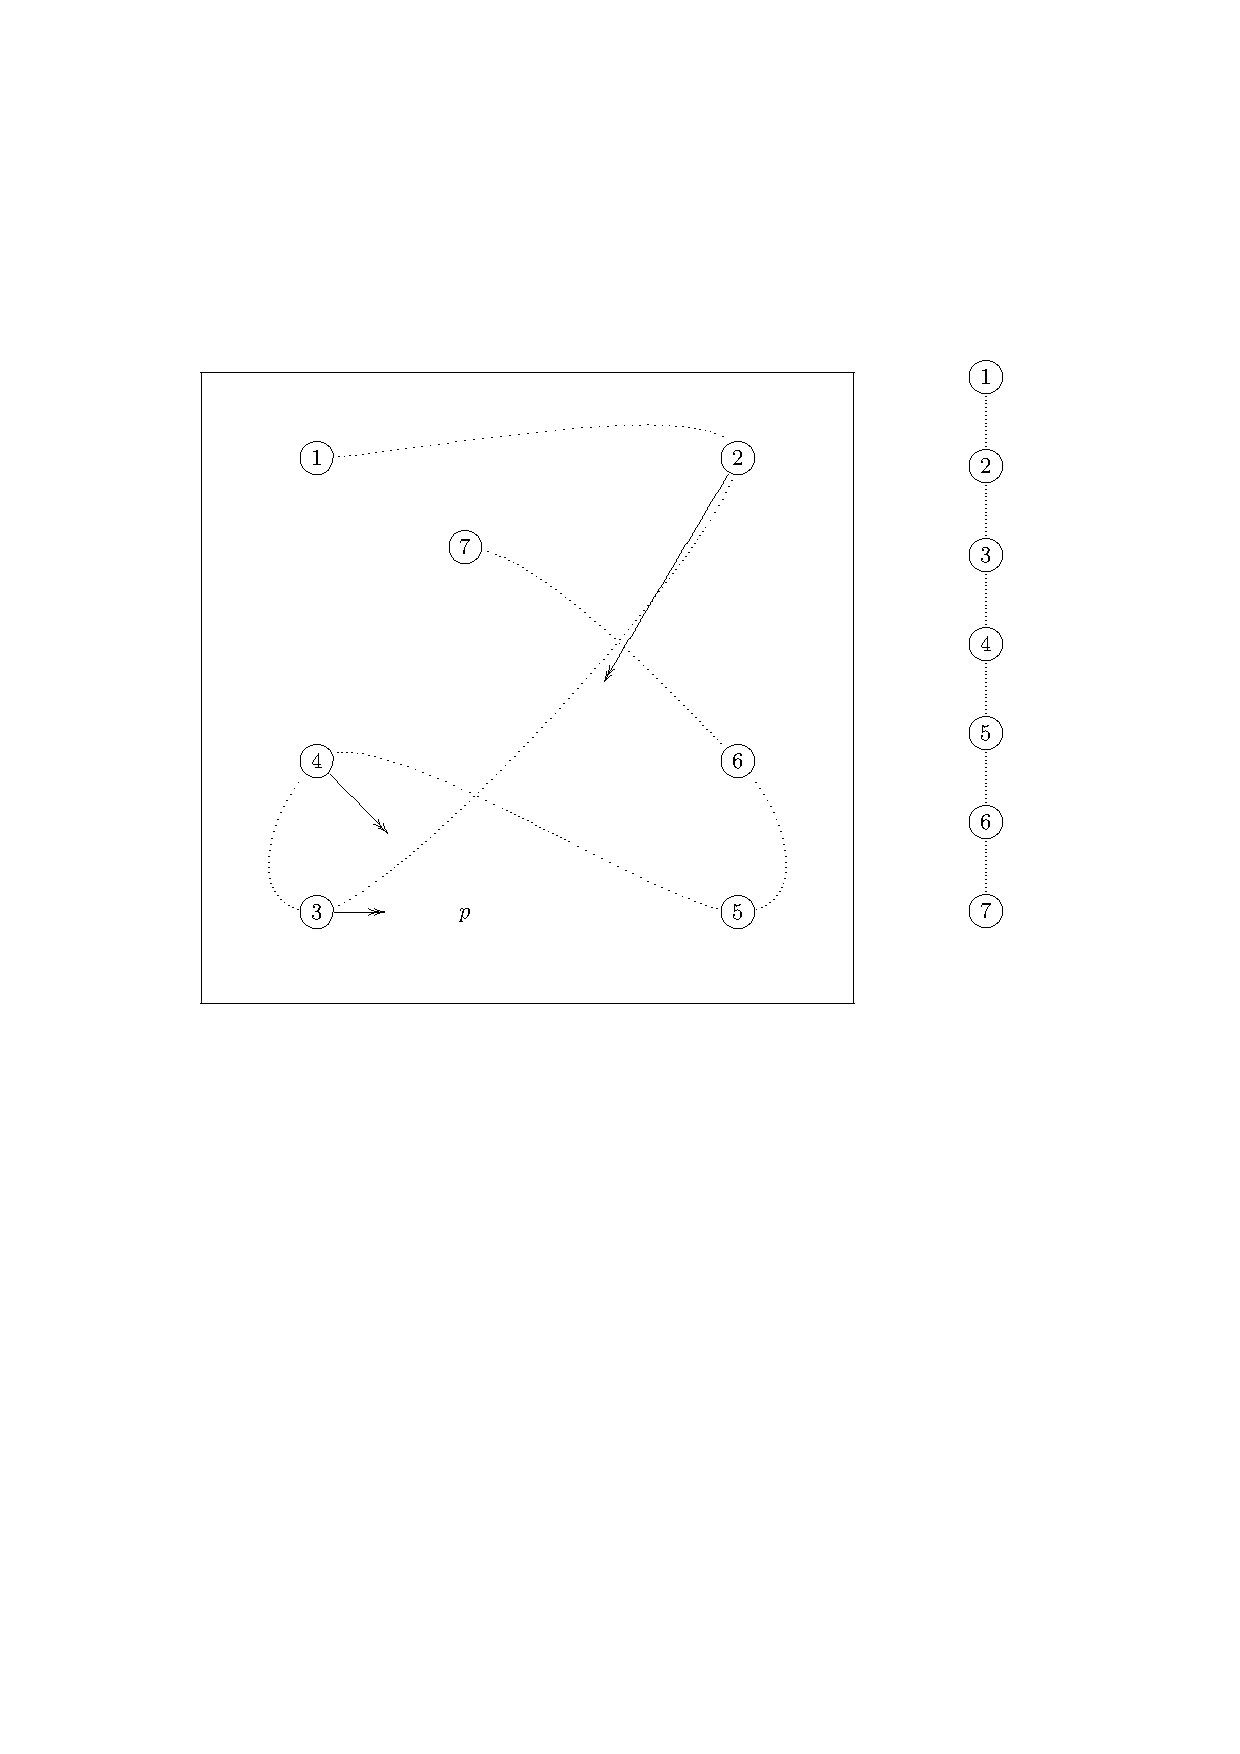
\includegraphics[width=\linewidth]{figures/ch08_som-training.pdf}
	\caption{Darstellung des zweidimensionalen Eingaberaumes (links) und des eindimensionalen Topologieraumes (rechts) einer SOM. Neuron 3 ist das Gewinnerneuron, da es $p$ am nächsten liegt. Die Nachbarn von Neuron 3 in der \emph{Topologie} sind die Neurone 2 und 4. Die Pfeile markieren die Bewegung des Gewinnerneurons und seiner Nachbarn in Richtung des Trainingsbeispiels $p$.}
	\label{fig:ch08_som-training}
\end{figure}

In Abbildung \ref{fig:ch08_som-training} wird ein beispielhafter Trainingsschritt abgebildet. Die eindimensionale Topologie der SOM ist zur Veranschaulichung durch die gepunkteten Linien in den Eingangsraum aufgetragen.

Obwohl das Zentrum von Neuron 7 vom \emph{Eingangsraum} aus gesehen wesentlich näher am Eingangsmuster $p$ liegt als das Neuron 2, lernt das Neuron 2, und das Neuron 7 nicht.
An dieser Stelle sei darauf hingewiesen, dass die \emph{Netztopologie} bestimmt, welches Neuron lernen darf und nicht die Lage im Eingangsraum.
Dies ist genau der Mechanismus, durch den eine Topologie einen Eingangsraum aussagekräftig abdecken kann, ohne mit ihm auf irgendeine Weise verwandt sein zu müssen.


\subsection*{Topologiefunktion}
Die Topologiefunktion $h(i,k,t)$ bestimmt, wie stark ein lernendes Neuron seine Nachbarn beeinflusst. Sie ist nicht auf dem Eingaberaum, sondern auf dem Gitter definiert und stellt die Nachbarschaftsbeziehung der SOM-Neuronen dar.

Prinzipiell ist der Sinn der Funktion, einen großen Wert anzunehmen, falls $k$ Nachbar des Gewinners oder gar der Gewinner selbst ist, und kleine Werte, falls nicht.
Schärfer definiert: Die Topologiefunktion muss \emph{unimodal} sein, also genau ein Maximum besitzen - dieses Maximum muss beim Gewinnerneuron $i$ liegen, das zu sich selbst natürlich die Entfernung $0$ hat.

Um große Werte für Nachbarn von $i$ und kleine Werte für Nicht-Nachbarn ausgeben zu können, braucht die Funktion $h$ eine Art \emph{Abstandsbegriff} auf dem Gitter. Dafür gibt es verschiedene Methoden (siehe Abbildung ).

\begin{figure}[ht!] \centering 
	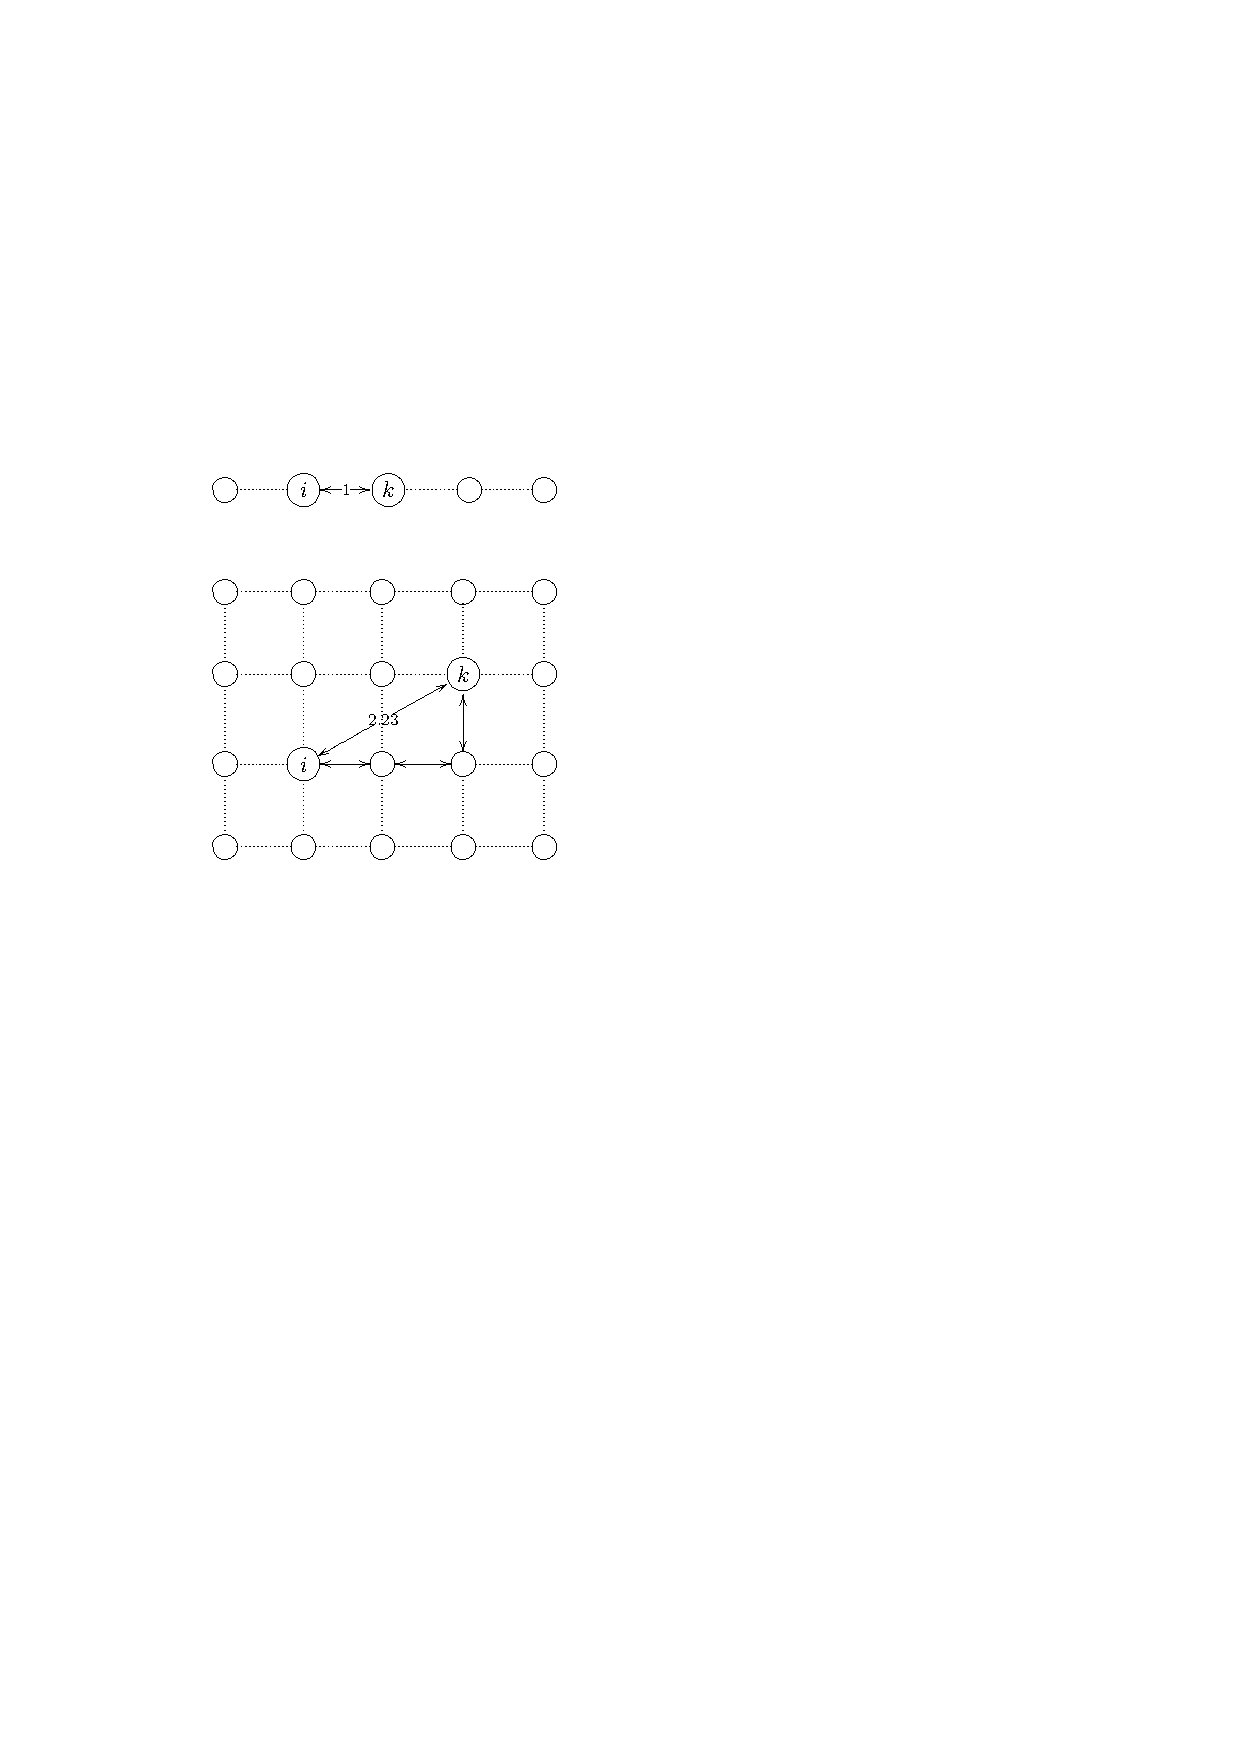
\includegraphics[width=0.5\linewidth]{figures/ch08_som-abstand-auf-gitter.pdf}
	\caption{Beispielabstände einer eindimensionalen (oben) und einer zweidimensionalen SOM-Topologie (unten) zwischen zwei SOM-Neuronen $i$ und $k$.}
	\label{fig:ch08_som-abstand-auf-gitter}
\end{figure}

Bei eindimensionalen Gittern kann die Anzahl der Verbindungen (diskrete Weglänge) zwischen $i$ und $k$ abgezählt werden.
Bei zweidimensionalen Gittern wird der Euklidische Abstand für die Abstandsberechnung herangezogen.

Eine \emph{Zeitabhängigkeit} ist optional, wird aber oft verwendet, um die Nachbarschaft mit der Zeit schrumpfen zu lassen.
Der Vorteil bei einer sinkenden Nachbarschaftsgröße ist, dass ein sich bewegendes Neuron zu Anfang viele Neurone in seiner Umgebung "`mitzieht"', sich das zufällig initialisierte Netz also am Anfang schnell und sauber entfalten kann.
Zum Ende des Lernvorganges hin werden nur noch wenige Neurone auf einmal beeinflusst, was das Netz im Gesamten steifer macht, aber ein gutes "`fine tuning"' der einzelnen Neurone ermöglicht.

\begin{figure}[ht!] \centering 
	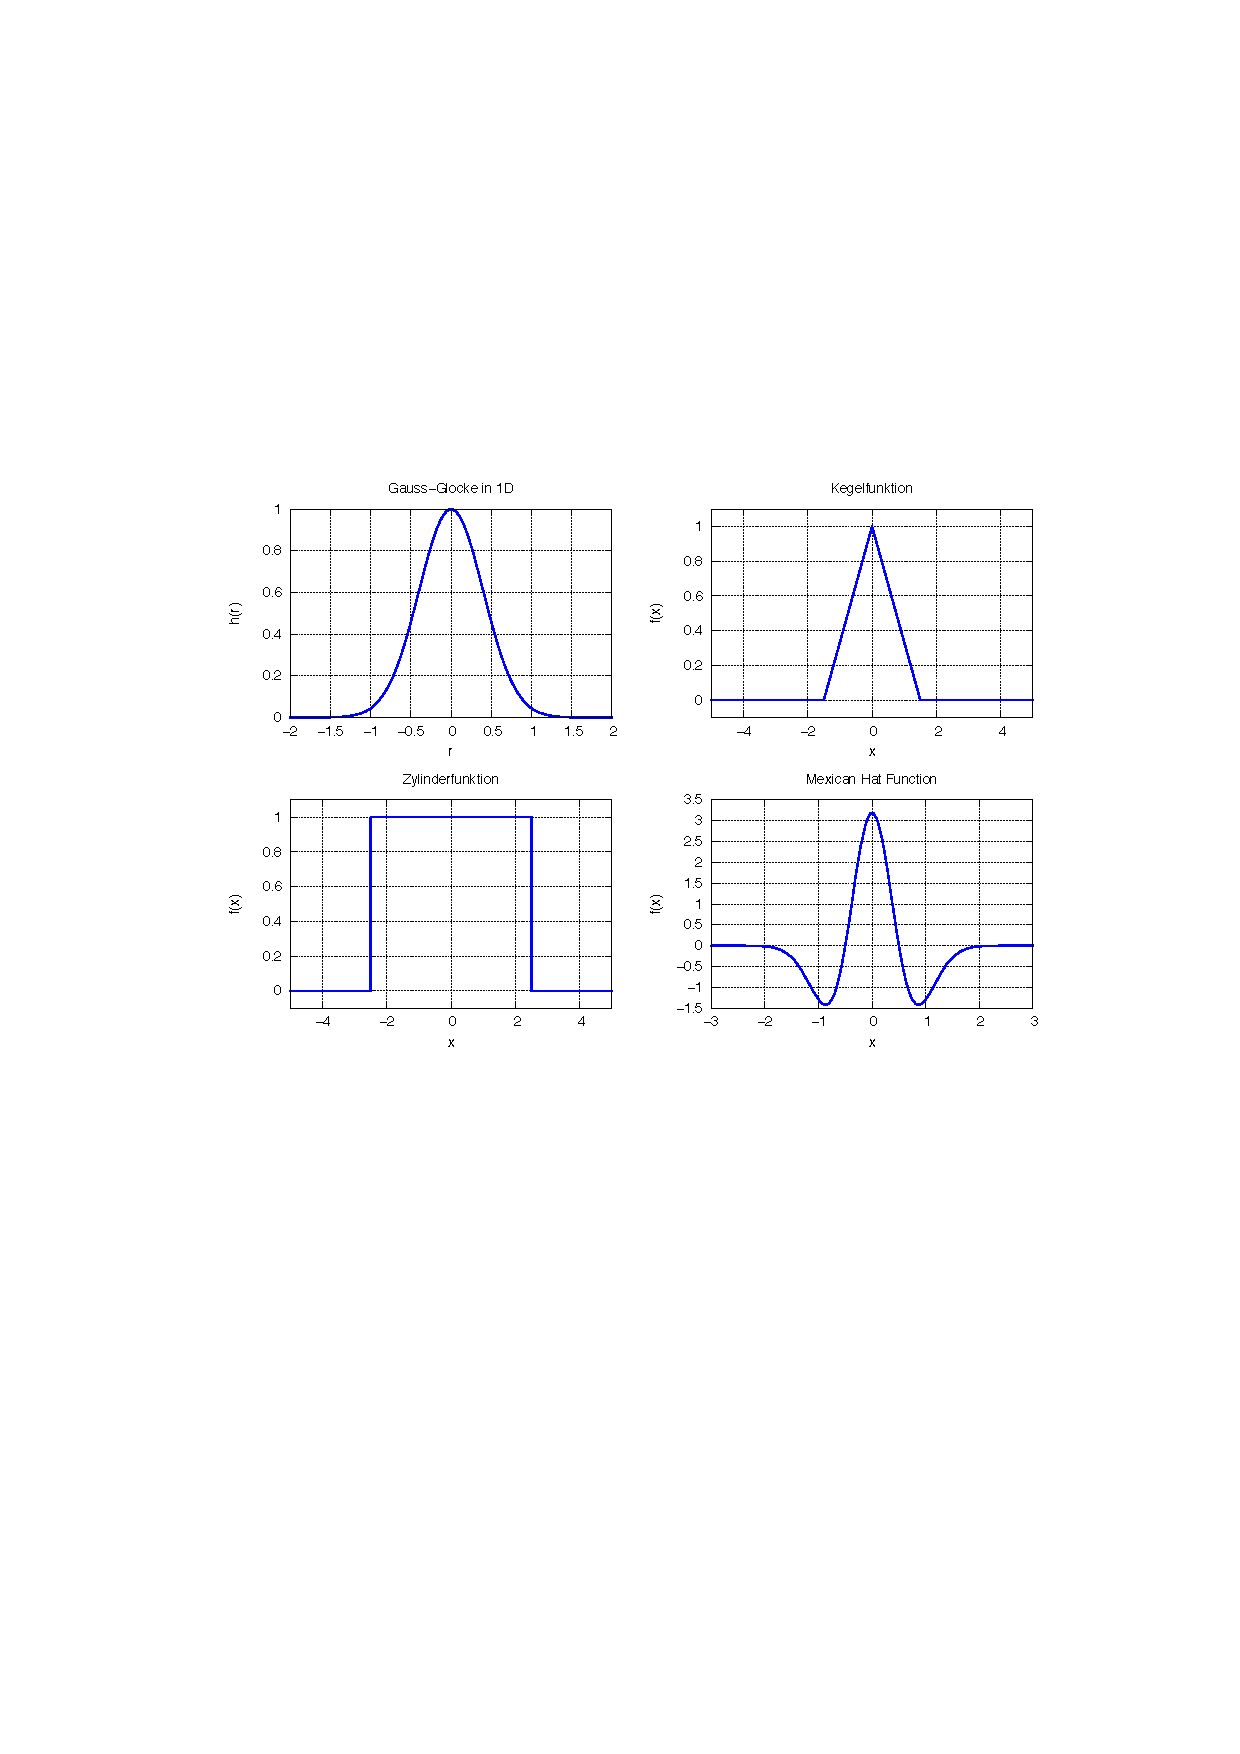
\includegraphics[width=\linewidth]{figures/ch08_som-topologiefunktionen.pdf}
	\caption{Mögliche Topologiefunktionen einer SOM: Gaußglocke, Kegelfunktion, Zylinderfunktion und die von Kohonen vorgeschlagene Mexican-Hat-Funktion.}
	\label{fig:ch08_som-topologiefunktionen}
\end{figure}


\subsubsection*{Gaußglocke}
Eine gängige Abstandsfunktion ist die \emph{Gaußglocke}. Sie ist unimodal mit einem Maximum bei 0 und kann zusätzlich durch den Parameter $\sigma$ in ihrer Breite verändert werden. Dies kann für die Realisierung der über die Zeit schrumpfenden Nachbarschaft genutzt werden.

Die Topologiefunktion hat dann die Form
\[
	h(i,k,t) = e^{\big(- \frac{||g_i - g_k||^2}{2 \cdot \sigma(t)^2}\big)}
\]
wobei $g_i$ und $g_k$ die Positionen der SOM-Neurone $i$ und $k$ \emph{auf dem Gitter}\footnote{Die Positionen im \emph{Eingaberaum} werden mit $c_i$ und $c_k$ bezeichnet.} bezeichnen.

\subsubsection*{Andere Topologiefunktionen}
Weitere Funktionen, die anstatt der Gaußfunktion eingesetzt werden können, sind zum Beispiel die Kegelfunktion, die Zylinderfunktion oder die Mexican-Hat-Funktion (siehe Abbildung \ref{fig:ch08_som-topologiefunktionen}).
Die Mexican-Hat-Funktion bietet hierbei eine besondere biologische Motivation: Sie stößt durch ihre negativen Stellen manche Neurone in der Umgebung des Gewinnerneurons ab, was man auch in der Natur schon beobachtet hat.
Dies kann für schärfere Abgrenzung der Kartenbereiche sorgen - genau aus diesem Grund wurde sie auch von Teuvo Kohonen selbst vorgeschlagen.


\subsection*{Entwicklung einer SOM}
Abbildung \ref{fig:ch08_som-entwicklung} zeigt wie sich eine eindimensionale SOM im zweidimensionalen Eingaberaum bei gleichverteilten Eingabemustern über die Zeit entwickeln kann.

\begin{figure}[ht!] \centering 
	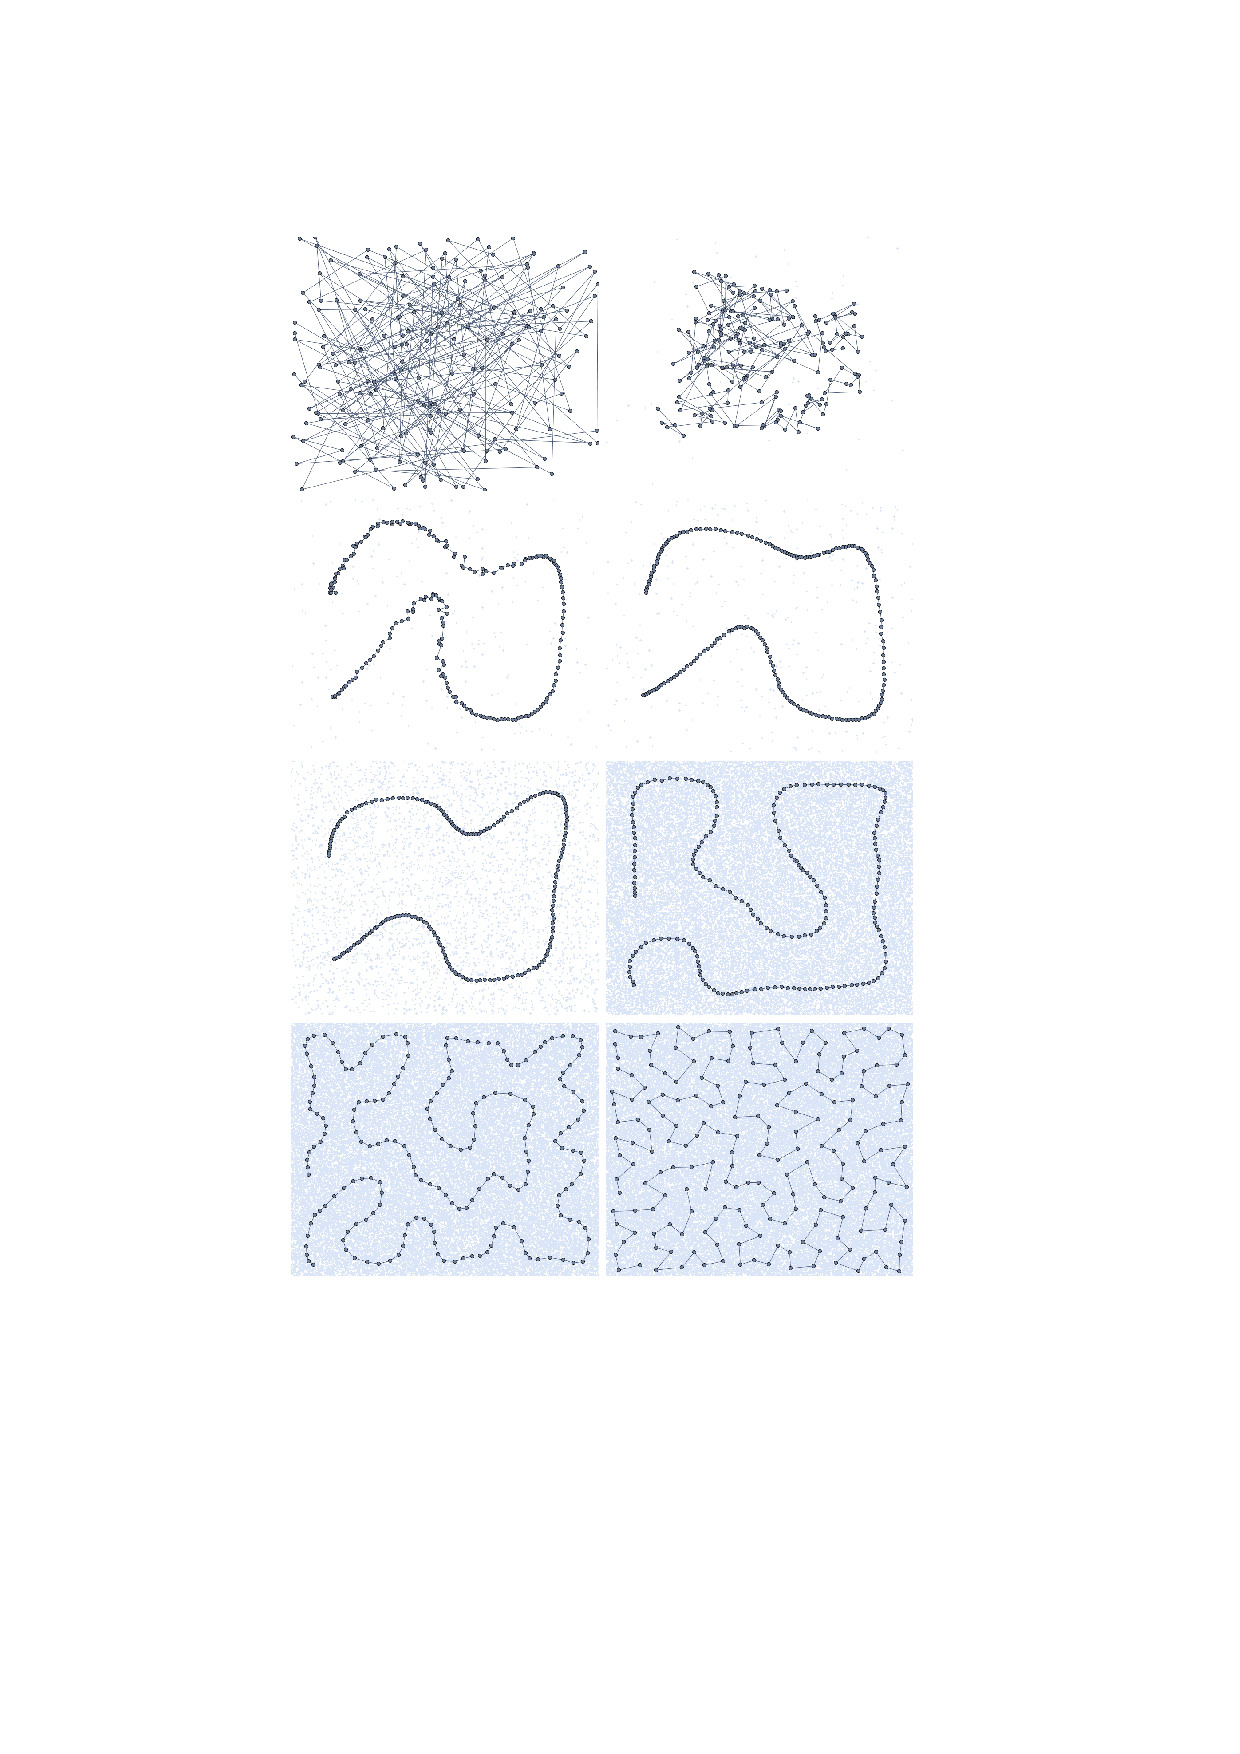
\includegraphics[width=\linewidth]{figures/ch08_som-entwicklung.pdf}
	\caption{Verhalten einer SOM mit eindimensionaler Topologie $(G = 1)$ nach Eingabe von 0, 100, 300, 500, 5000, 50000, 70000 und 80000 zufällig verteilten Eingabemustern $p \in R^2$. $\eta$ fiel während des Trainings von 1.0 auf 0.1, der $\sigma$-Parameter der als Nachbarschaftsmaß eingesetzten Gauß-Funktion von 10.0 auf 0.2.}
	\label{fig:ch08_som-entwicklung}
\end{figure}

In Abbildung \ref{fig:ch08_som-endzustaende} sind Endzustände von ein- und zweidimensionalen SOMs bei verschieden geformten Eingaberäumen zu sehen. Dabei wird deutlich, dass nicht alle Eingaberäume durch jede Netztopologie gut abgedeckt werden. Es gibt sogenannte \emph{freiliegende} Neurone, Neurone welche in einem Bereich liegen, in dem kein Inputmuster je aufgetreten ist.

Eine eindimensionale Topologie produziert in der Regel weniger solcher freiliegenden Neuronen.

\begin{figure}[ht!] \centering 
	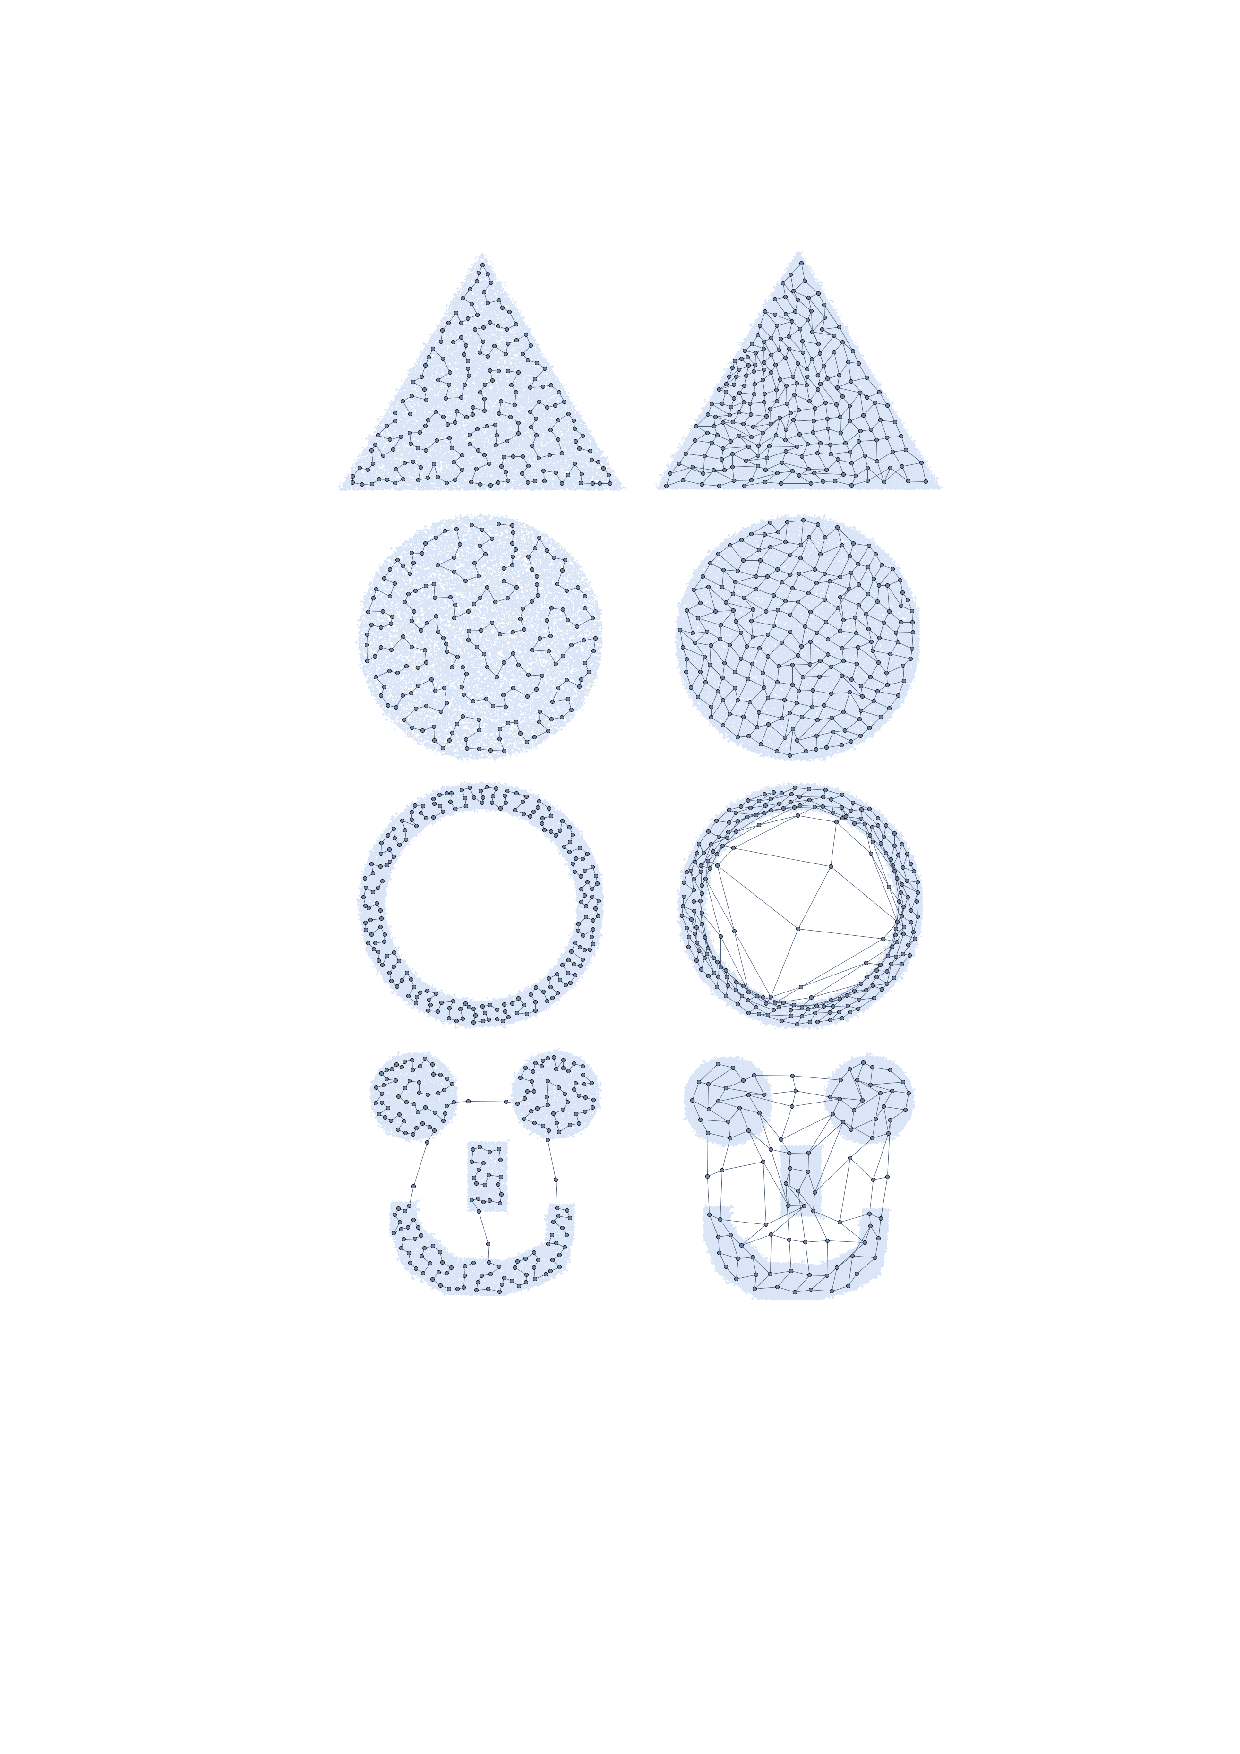
\includegraphics[width=\linewidth]{figures/ch08_som-endzustaende.pdf}
	\caption{Endzustände von eindimensionalen (linke Spalte) und zweidimensionalen (rechte Spalte) SOMs auf verschieden abgedeckten Eingaberäumen. Genutzt wurden bei eindimensionaler Topologie 200 Neuronen, bei zweidimensionaler 10 $\times$ 10 Neurone und bei allen Karten 80.000 Eingabemuster.}
	\label{fig:ch08_som-endzustaende}
\end{figure}

